\begin{filecontents*}{mybib.bib}
@book{Sutton2018,
  added-at = {2019-07-13T10:11:53.000+0200},
  author = {Sutton, Richard S. and Barto, Andrew G.},
  biburl = {https://www.bibsonomy.org/bibtex/2f46601cf8b13d39d1378af0d79438b12/lanteunis},
  edition = {Second},
  interhash = {ac6b144aaec1819919a2fba9f705c852},
  intrahash = {f46601cf8b13d39d1378af0d79438b12},
  keywords = {},
  publisher = {The MIT Press},
  timestamp = {2019-07-13T10:11:53.000+0200},
  title = {Reinforcement Learning: An Introduction},
  url = {http://incompleteideas.net/book/the-book-2nd.html},
  year = {2018 }
}
\end{filecontents*}

\documentclass[10pt,a4paper]{article}
\usepackage[utf8]{inputenc}
\usepackage[top=1.25in, bottom=1.25in, left=.75in, right=.75in]{geometry}
\usepackage{amsmath}
\usepackage{amsfonts}
\usepackage{mathtools}
\usepackage{amssymb}
\usepackage{xcolor}
\usepackage{natbib}
\usepackage{bibentry}
\usepackage{fancyhdr}
\pagestyle{fancy}
\lhead{Exercise sheet \#1}
\nobibliography*
\DeclareMathOperator*{\argmax}{arg\,max}
\author{Johannes Ender}
\begin{document}
\section{Multiarmed Bandits}
\subsection*{1. Exercise 2.1 In $\epsilon$-greedy action selection, for the case of two actions and $\epsilon$ = 0.5, what is the probability that the greedy action is selected?}
An $\epsilon$ value of 0.5 means, that in 50 percent of the cases, the greedy action is taken. But, as in the $\epsilon$ there is also a probability of 0.5 of the greedy action being taken, the actual probability is higher:
\begin{align*}
p(a_{greedy}) = 1 - 0.5 + \frac{0.5}{2} = 0.75
\end{align*}

\subsection*{2. Exercise 2.2 Bandit example Consider a k-armed bandit problem with k = 4 actions, denoted 1, 2, 3, and 4. Consider applying to this problem a bandit algorithm using $\epsilon$-greedy action selection, sample-average action-value estimates, and initial estimates of $Q_1 (a) = 0$, for all a. Suppose the initial sequence of actions and rewards is $A_1 = 1, R_1 = 1, A_2 = 2, R_2 = 1, A_3 = 2, R_3 = 2, A_4 = 2, R_4 = 2, A_5 = 3, R_5 = 0$. On some of these time steps the $\epsilon$ case may have occurred, causing an action to be selected at random. On which time steps did this definitely occur? On which time steps could this possibly have occurred?}

\begin{center}
\begin{table}[ht]
\centering
\begin{tabular}{|c|c|c|c|c|c|c|}
\hline 
a & $Q_1(a)$ & $Q_2(a)$ & $Q_3(a)$ & $Q_4(a)$ & $Q_5(a)$ & $Q_6(a)$ \\ 
\hline 
$A_1$ & 0 & \textcolor{red}{1} & \textcolor{red}{1} & 1 & 1 & 1 \\ 
\hline 
$A_2$ & 0 & 0 & \textcolor{red}{1} & \textcolor{red}{1.5} & \textcolor{red}{1.67} & \textcolor{red}{1.67} \\ 
\hline 
$A_3$ & 0 & 0 & 0 & 0 & 0 & 0 \\ 
\hline 
$A_4$ & 0 & 0 & 0 & 0 & 0 & 0 \\ 
\hline 
\end{tabular} 
\caption{\textcolor{red}{red} color indicates the $\operatorname*{argmax}_a Q_t(a)$}
\end{table}
\end{center}
Time steps, where $\epsilon$-choice \textbf{definitely} occurred:
\begin{itemize}
\item 2 $\rightarrow$: maximum estimate would be $A_1$, but $A_2$ was chosen
\item 5 $\rightarrow$: $A_2$ would have the highest estimated value, but $A_3$ is chosen
\end{itemize}
Time steps, where $\epsilon$-choice \textbf{possibly} occurred:
\begin{itemize}
\item 1 $\rightarrow$: there is no maximum value in the estimates, has to be randomly chosen, but could also have been a random choice caused by an $\epsilon$ case	
\item 3 $\rightarrow$: $A_1$ and $A_2$ have the same estimate value and a random choice has to be made, but could also have been a random choice caused by an $\epsilon$ case
\item 4 $\rightarrow$: the action with the highest estimated value is chosen, but since in the $\epsilon$ case, the random choice is made between all actions, this could also possibly be an $\epsilon$ case
\end{itemize}
\subsection*{3. Exercise 2.3 In the comparison shown in Figure 2.2 (below), which method will perform best in the long run in terms of cumulative reward and probability of selecting the best action? How much better will it be? Express your answer quantitatively.}
The $\epsilon$-greedy strategy in the long run converges to taking the optimal action in $(1-\epsilon) \cdot 100 = 90$ \% of the cases, which is higher than the $\sim 80$ \% the optimistic strategy seems to converge to.
\newpage
\subsection*{4. Implementation Task: 10 armed-testbed}
\begin{figure}[h]
\centering
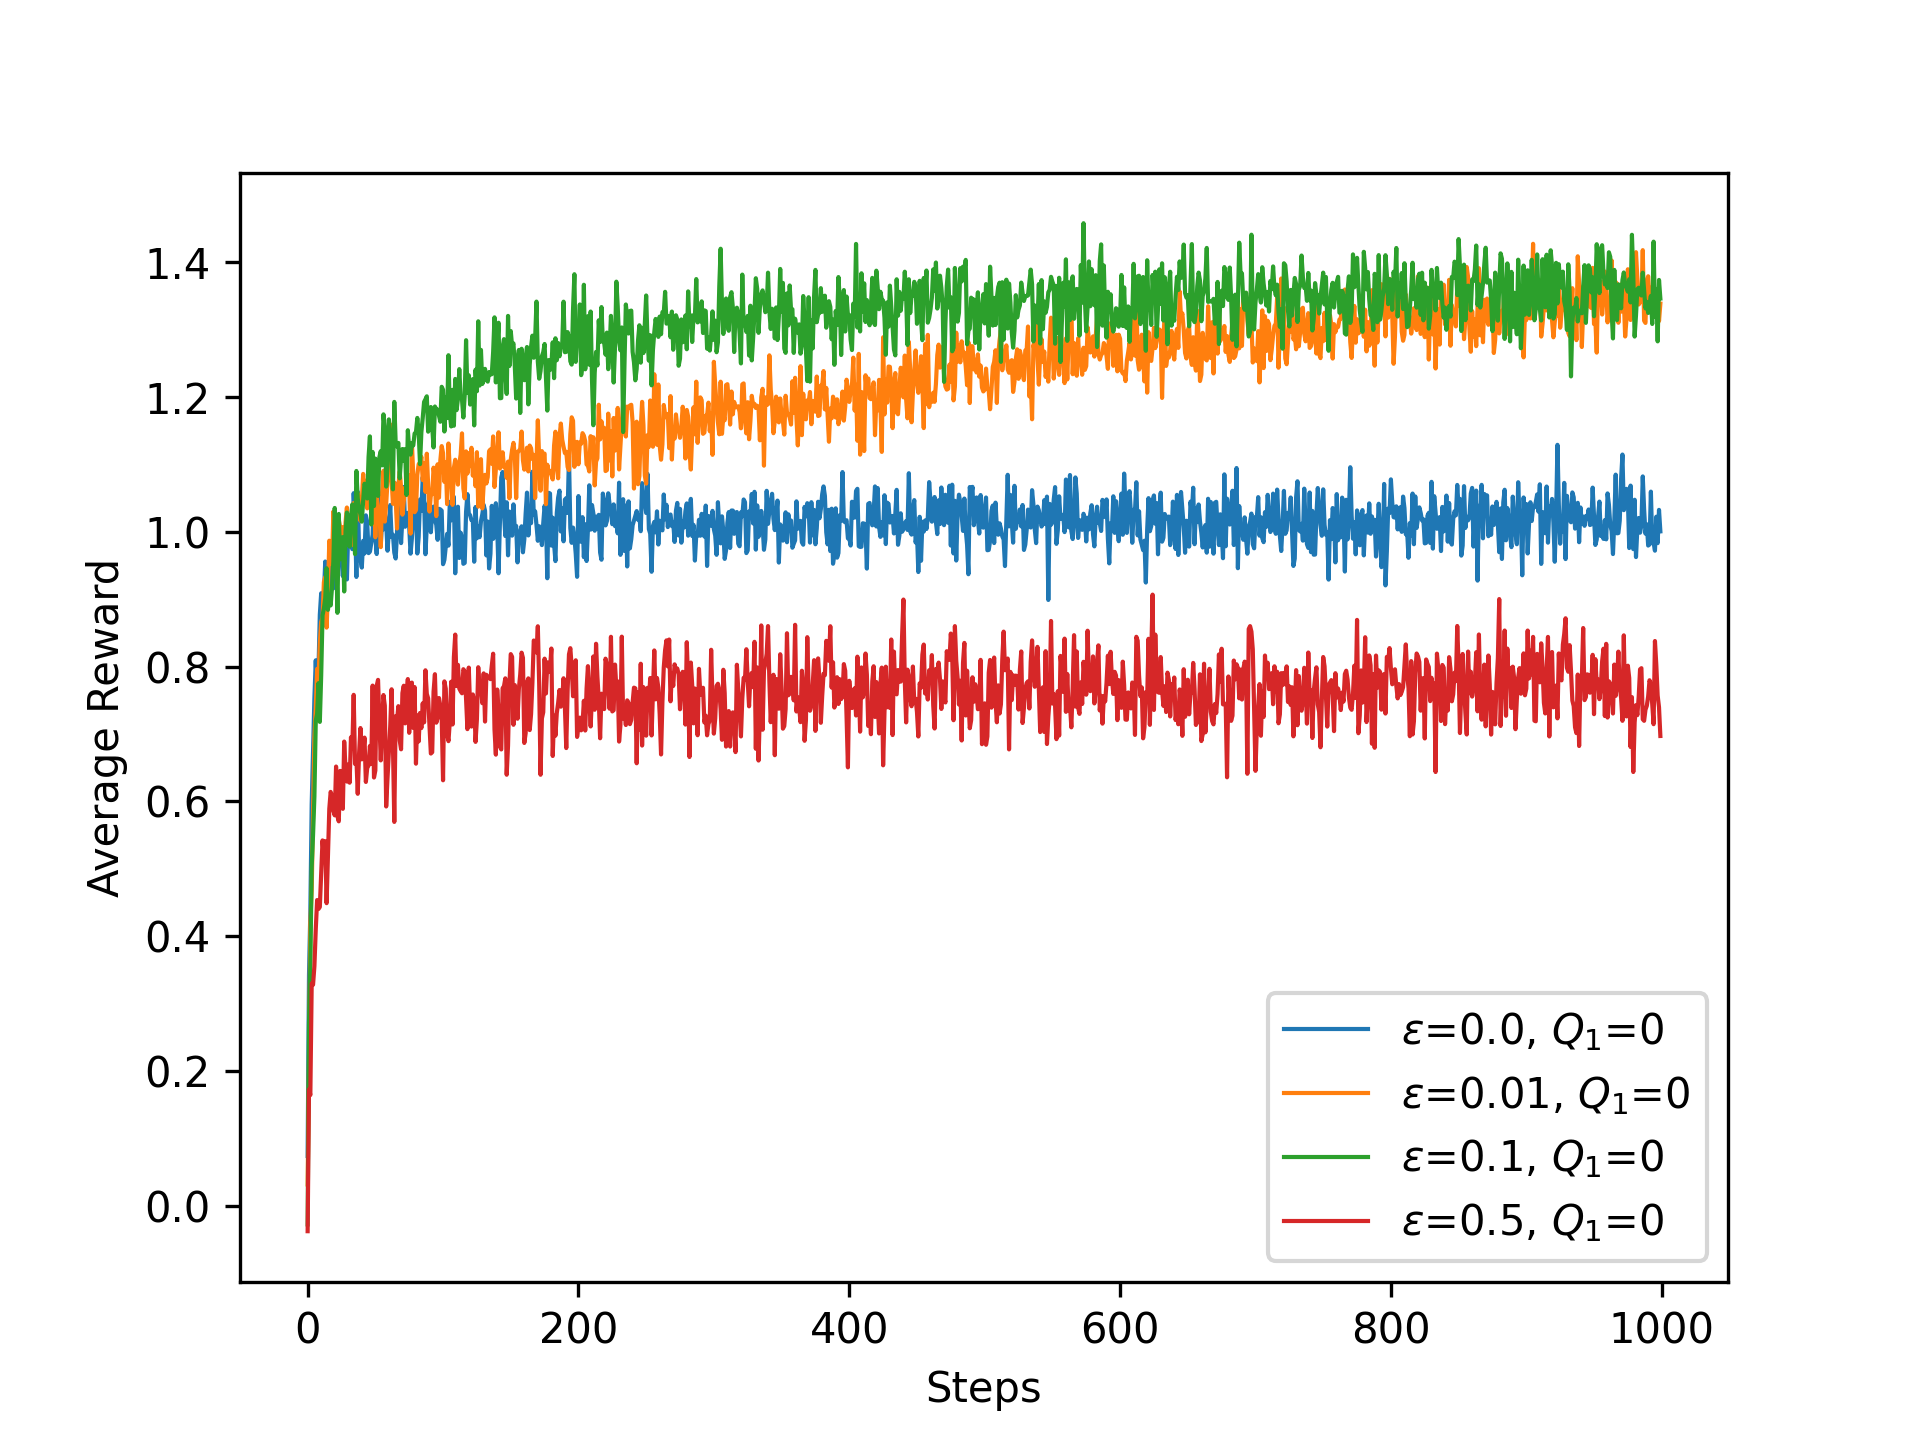
\includegraphics[width=0.6\linewidth]{./averageReward.png}
\caption{Average reward for 1000 time steps averaged over 1000 runs for various $\epsilon$ values.}
\end{figure}
\begin{figure}[h]
\centering
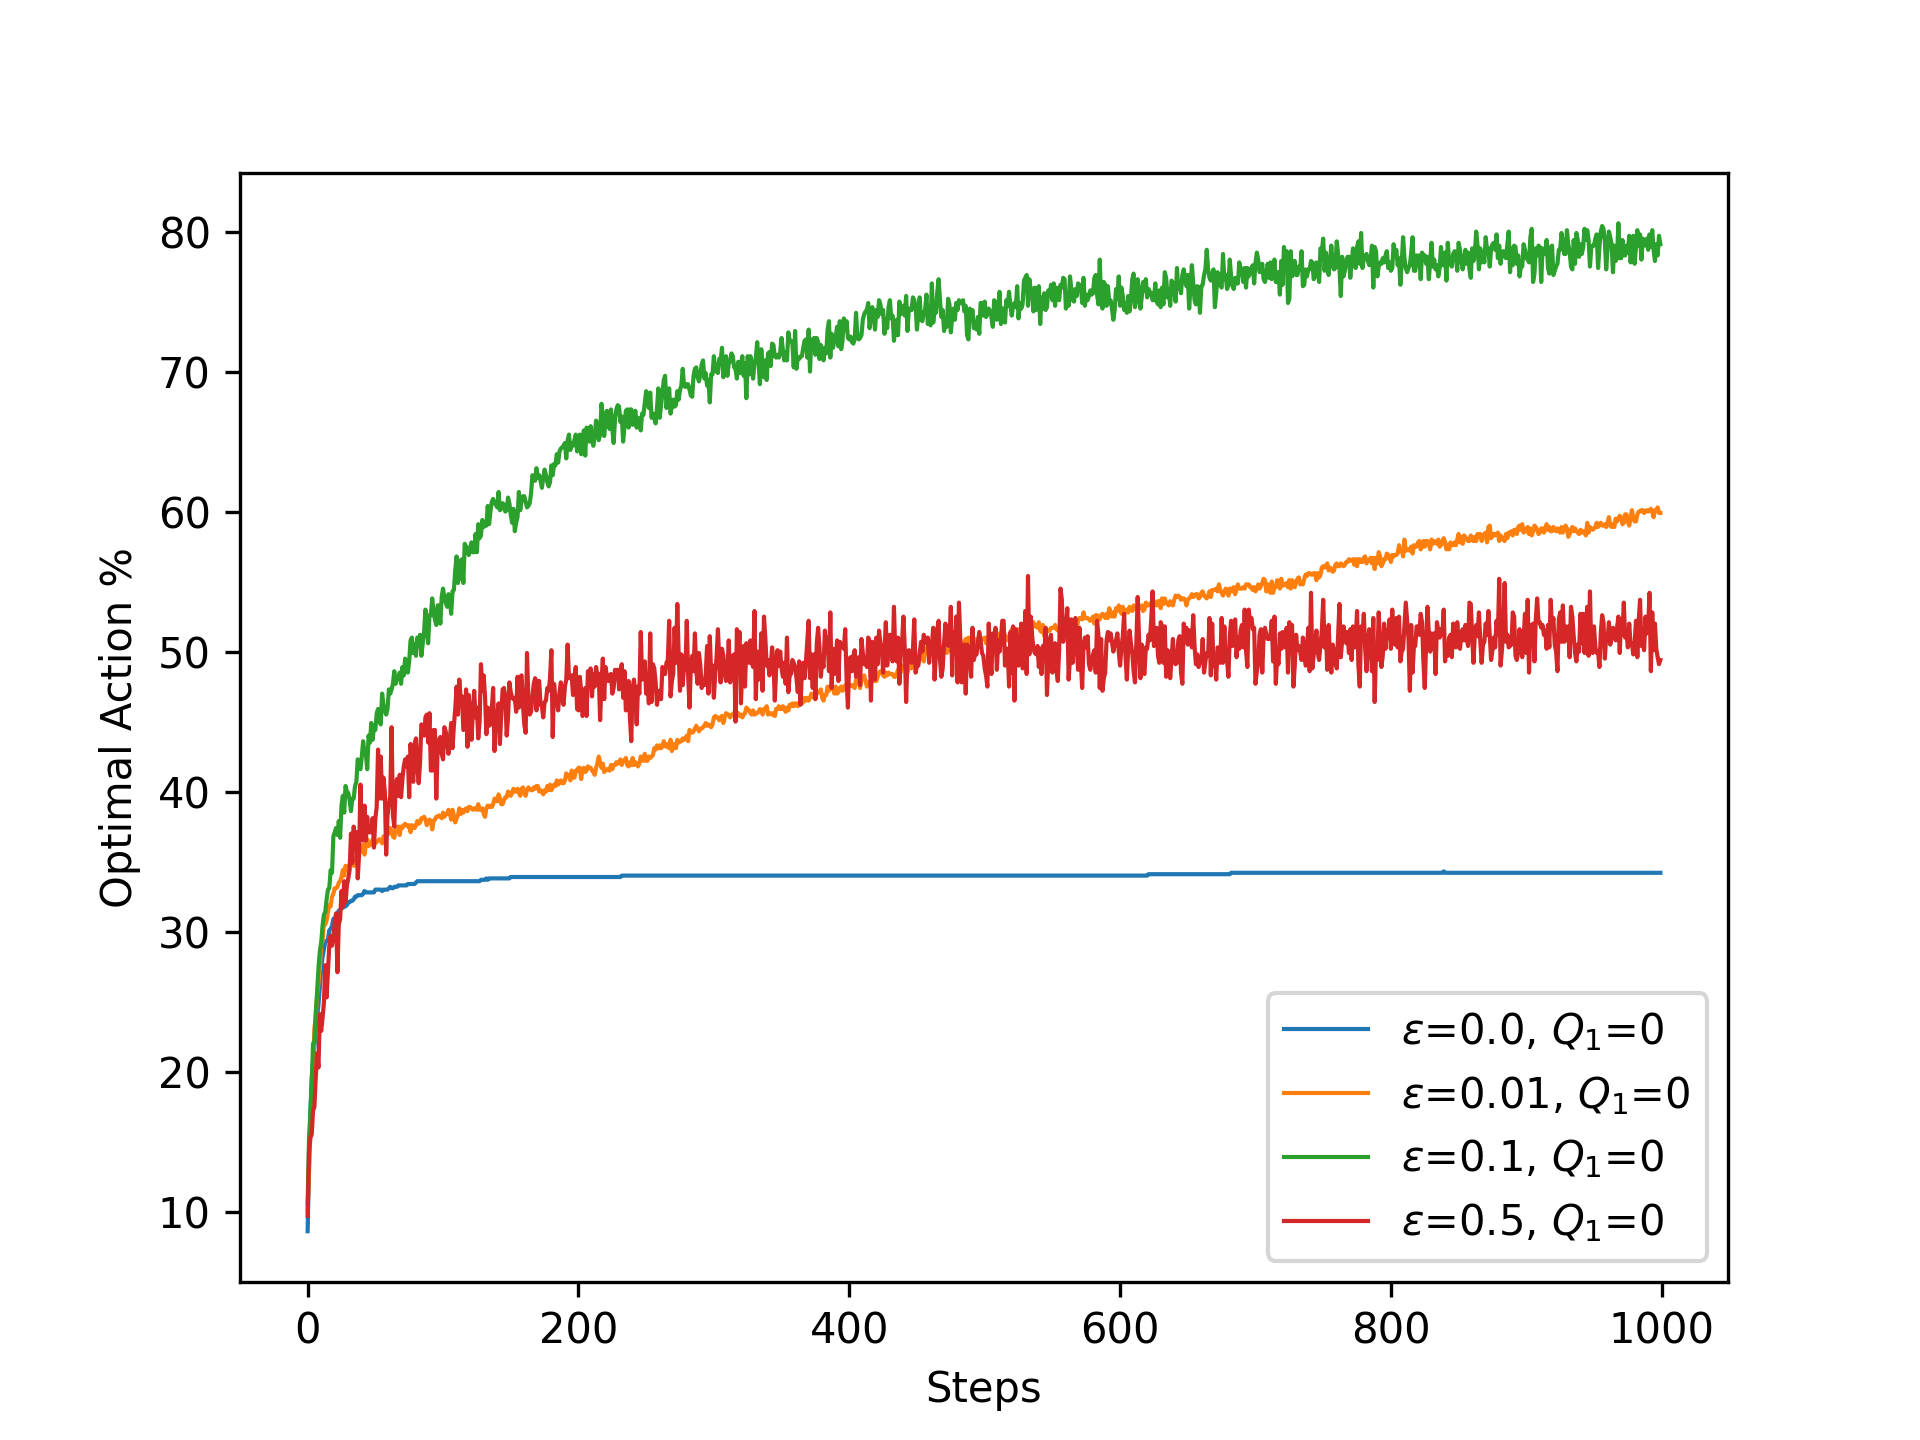
\includegraphics[width=0.6\linewidth]{./optimalAction.png}
\caption{Percentage of optimal action chosen for 1000 time steps averaged over 1000 runs for various $\epsilon$ values.}
\end{figure}
\newpage
\subsection*{5. Exercise 2.4 If the step-size parameters, $\alpha_n$ , are not constant, then the estimate $Q_n$ is a weighted average of previously received rewards with a weighting different from that given by (2.6). What is the weighting on each prior reward for the general case, analogous to (2.6), in terms of the sequence of step-size parameters?}
\begin{align*}
G_{n+1} &= Q_n + \alpha_n [R_n - Q_n] \\
&= \alpha_n R_n + (1 - \alpha_n)Q_n \\
&= \alpha_n R_n + (1 - \alpha_n)[\alpha_{n-1} R_{n-1} + (1-\alpha_{n-1})Q_{n-1}] \\
&= \alpha_n R_n + (1 - \alpha_n)\alpha_{n-1} R_{n-1} + (1 - \alpha_{n})(1 - \alpha_{n-1})Q_{n-1} \\
&= Q_1 \prod_{k=1}^{n} (1- \alpha_k) + \sum_{i = 1}^n R_i \alpha_i \prod_{k = i + 1}^n (1 - \alpha_k)
\end{align*}
\subsection*{6. Exercise 2.6 Mysterious Spikes\\The results shown in Figure 2.3 should be quite reliable because they are averages over 2000 individual, randomly chosen 10-armed bandit tasks. Why, then, are there oscillations and spikes in the early part of the curve for the optimistic method? In other words, what might make this method perform particularly better or worse, on average, on particular early steps?}
The method with optimistic initial estimates is good to encourage the agent to explore more in the beginning. When all the estimates are initialized relatively large, the agent will continue choosing one of the not yet chosen actions, since the estimate will be lower after being chosen once, as the initial values are above the true value.\\
This initial encouragement for exploration of course also leads to non-optimal choices, which explains the slower rise in optimal action selection compared to the realistic agent.

\newpage
\section{Markov Decision Processes}
\subsection*{7. Exercise 3.2 Is the MDP framework adequate to usefully represent all goal-directed learning tasks? Can you think of any clear exceptions?}
An example would be driving with your bike (or car) from a point A to a point B such that the distance or duration are minimized.
If all the streets were empty, the task could be represented by the MDP framework, but in a realistic scenario there also other road users and a route that on one day is the shortest or fastest route, but on the next day there is a traffic jam or maybe a construction site, such that a certain road on this route cannot be taken at all. \\
So, I guess all tasks where there are unpredictable events, like other agents with potentially interfering goals (other road users or a construction site blocking a road), are not well represented by the MDP framework.

\subsection*{8. Exercise 3.4 Give a table analogous to that in Example 3.3 (textbook p. 52), but for p(s' , r $\mid$ s, a). It should have columns for s, a, s' , r, and p(s' , r $\mid$ s, a), and a row for every 4-tuple for which p(s', r $\mid$  s, a) $>$ 0.}
The table basically stays the same as in the textbook on page 52, but without the rows containing p(s' $\mid$ s, a) = 0. This is due to the fact that the probability of performing the transition from state $s$ to state $s'$ stays the same, irrespective of the reward.
\begin{center}
\begin{table}[ht]
\centering
\begin{tabular}{|c|c|c|c|c|}
\hline 
s & a & s' & r(s, a, s') & p(s', r $\mid$ s, a) \\ 
\hline 
\hline
\texttt{high} & \texttt{search} & \texttt{high} & \texttt{$r_{search}$} & $\alpha$ \\ 
\hline 
\texttt{high} & \texttt{search} & \texttt{low} & \texttt{$r_{search}$} & 1 - $\alpha$ \\ 
\hline 
\texttt{low} & \texttt{search} & \texttt{high} & -3 & 1 - $\beta$ \\ 
\hline 
\texttt{low} & \texttt{search} & \texttt{low} & \texttt{$r_{search}$} & $\beta$ \\ 
\hline 
\texttt{high} & \texttt{wait} & \texttt{high} & \texttt{$r_{wait}$} & 1 \\ 
\hline 
\texttt{low} & \texttt{wait} & \texttt{low} & \texttt{$r_{wait}$} & 1 \\ 
\hline 
\end{tabular}
\end{table}
\end{center}

\subsection*{9. Exercise 3.6 Suppose you treated pole-balancing as an episodic task but also used discounting, with all rewards zero except for -1 upon failure. What then would the return be at each time? How does this return differ from that in the discounted, continuing formulation of this task?}
Assuming each episode takes k time steps and all rewards being zero except the reward on failure being -1, the discounted return would be:
$$
G_t = R_{t+1} + \gamma R_{t+2} + \gamma^2R_{t+2} + \cdots = 0 + \gamma 0 + \gamma^2 0 \cdots + \gamma^k \cdot (-1) = -\gamma^k
$$
This is the same expected return as for the continuing task. The difference is that there can also be episodes where failure does not occur in which case the return would be zero.

\subsection*{10. Exercise 3.7 Imagine that you are designing a robot to run a maze. You decide to give it a reward of +1 for escaping from the maze and a reward of zero at all other times. The task seems to break down naturally into episodes - the successive runs through the maze - so you decide to treat it as an episodic task, where the goal is to maximize expected total reward (3.7). After running the learning agent for a while, you find that it is showing no improvement in escaping from the maze. What is going wrong? Have you effectively communicated to the agent what you want it to achieve?}
The problem here is that the agent gets the reward no matter how long it takes him to escape the maze. The given formulation of the task just tells the agent that it should escape, but not that it should find the shortest way out. A better formulation could be to give the agent a reward of -1 for every time step where it does not escape and a reward of 0/+1 for the escape. Like this, it would try to minimize the negative rewards and thus learn a shorter way out of the maze.

\subsection*{11. Exercise 3.8 Suppose $\gamma$ = 0.5 and the following sequence of rewards is received $R_1$ = -1, $R_2$ = 2, $R_3$ = 6, $R_4$ = 3, and $R_5$ = 2, with T = 5. What are $G_0$ , $G_1$ , . . ., $G_5$ ? Hint: Work backwards.}
Using the general formula $G_t = R_{t+1} + \gamma G_{t+1}$:
$$G_5 = 0$$
$$G_4 = R_5 + 0.5 \cdot G_5 = 2 + 0.5 \cdot 0 = 2$$
$$G_3 = R_4 + 0.5 \cdot G_4 = 3 + 0.5 \cdot 2 = 4$$
$$G_2 = R_3 + 0.5 \cdot G_3 = 6 + 0.5 \cdot 4 = 8$$
$$G_1 = R_2 + 0.5 \cdot G_2 = 2 + 0.5 \cdot 8 = 6$$
$$G_0 = R_1 + 0.5 \cdot G_1 = -1 + 0.5 \cdot 6 = 2$$

\subsection*{12. Exercise 3.9 Suppose $\gamma$ = 0.9 and the reward sequence is $R_1$ = 2 followed by an infinite sequence of 7s. What are $G_1$ and $G_0$ ?}
$G_1$ can be calculated as
\begin{align*}
G_1 &= R_2 + \gamma \cdot G_2 \\&= R_2 + \gamma \cdot R_3 + \gamma^2 \cdot R_4 + \gamma^3 \cdot R_5 + \cdots \\
 	&= 7 + \gamma \cdot 7 + \gamma^2 \cdot 7 + \gamma^3 \cdot 7 + \cdots \\
\end{align*}
Here, one can make use of formula 3.10 on page 55 of \cite{Sutton1998} and reformulate to:
\begin{align*}
G_1 &= 7 \cdot \sum_{k=0}^\infty \\&= 7 \cdot \frac{1}{1 - \gamma} \\&= 7 \cdot \frac{1}{0.1} \\&= 7 \cdot 10 = 70 \\
\end{align*}
and using this result one can calculate $G_0$:
\begin{align*}
G_0 = R_1 + \gamma G_1 = 2 + 0.9 \cdot 70 = 65
\end{align*}

\subsection*{13. Exercise 3.11 If the current state is $S_t$, and actions are selected according to stochastic policy $\pi$ , then what is the expectation of $R_{t+1}$ in terms of $\pi$ and the four-argument function p (3.2)?}
\begin{align*}
\mathbb{E}[R_{t+1} \mid s=S_t] &= \sum_a \pi(a \mid s) \sum_r r \sum_{s' \epsilon \mathcal{S}} p(s', r \mid s, a) \\
&= \sum_a \pi(a \mid s) \sum_{r, s'} r p(s', r \mid s, a)
\end{align*}

\subsection*{14. Exercise 3.14 The Bellman equation (3.14) must hold for each state for the value function $v_\pi$ shown in Figure 3.2 (right) of Example 3.5. Show numerically that this equation holds for the center state, valued at +0.7, with respect to its four neighboring states, valued at +2.3, +0.4, -0.4, and +0.7. (These numbers are accurate only to one decimal place.)}
Using the Bellman equation
\begin{align*}
v_\pi (s) = \sum_a \pi (a \mid s) \sum_{r, s'} p(s', r \mid s, a)[r + \gamma v_\pi (s')]
\end{align*}
and $\mathcal{A}(s) = \{\texttt{north, south, east, west}\}, \mathcal{S} = \{s_{north}, s_{south}, s_{east}, s_{west}\}, \gamma = 0.9 and r = 0$ (since there is no transition away from a special state or off the grid), one can calculate the value of the central state as:
\begin{align*}
v_\pi(s_{central}) = &\frac{1}{4} \cdot 1 \cdot 0.9 \cdot 2.3 + \quad \quad \quad &\backslash \backslash \quad \texttt{north} \\
&\frac{1}{4} \cdot 1 \cdot 0.9 \cdot 0.4 + &\backslash \backslash \quad \texttt{east} \\
&\frac{1}{4} \cdot 1 \cdot 0.9 \cdot (-0.4) + &\backslash \backslash \quad \texttt{south} \\
&\frac{1}{4} \cdot 1 \cdot 0.9 \cdot 0.7 &\backslash \backslash \quad \texttt{west} \\
&= 0.675
\end{align*}
Since taking an action deterministically moves the agent in the according direction, the probability of e.g. reaching state $s_{east}$ after taking action $\texttt{east}$ is 1 and 0 for all other states. Thus, all these cases contribute nothing to the value calculation and since there is only one reward (0), only the four cases for the four different actions need to be considered.

\subsection*{15. Exercise 3.15 In the gridworld example, rewards are positive for goals, negative for running into the edge of the world, and zero the rest of the time. Are the signs of these rewards important, or only the intervals between them? Prove, using (3.8), that adding a constant c to all the rewards adds a constant, v c , to the values of all states, and thus does not affect the relative values of any states under any policies. What is $v_c$ in terms of c and $\gamma$?}
Adding a constant to equation (3.8) results in:
\begin{align*}
G_t &= \sum_{k=0}^\infty \gamma^k (R_{t+k+1} + c) \\
&= \underbrace{\sum_{k=0}^\infty \gamma^k\; R_{t+k+1}}_{v_\pi} + \underbrace{\sum_{k=0}^\infty \gamma^k\; c}_{v_c}
\end{align*}
$v_c$ does not depend on the current state and can be calculated as
\begin{align*}
v_c = \sum_{k=0}^\infty \gamma^k\; c = \frac{c	}{1 - \gamma}
\end{align*}


\subsection*{16. Exercise 3.16 Now consider adding a constant c to all the rewards in an episodic task, such as maze running. Would this have any effect, or would it leave the task unchanged as in the continuing task above? Why or why not? Give an example.}
Using the finite series summation formula
\begin{align*}
\sum_{k=0}^{n} = \frac{1-z^{n+1}}{1-z}
\end{align*}
one can show that the additional expected reward due to the addition of a constant would depend on the length of the episode (assuming the episode length is not fixed).
The expected value of a state
\begin{align*}
v_c=\sum_{k=0}^{t_{final}-t} c \cdot \gamma^k = c \cdot \frac{1 - \gamma^{t_{final}-t+1}}{1 - \gamma}
\end{align*}
The summation goes from $0$ to $t_{final}-t$ as it has to sum over the steps remaining in the current episode. \\
If $t_{final} = 20,\; t = 0\; \gamma=0.9$:
\begin{align*}
v_c= c \cdot \frac{1 - 0.9^{21}}{1- 0.9} = c \cdot 8.9
\end{align*}
If $t_{final} = 40,\; t=0\; \gamma=0.9$:
\begin{align*}
v_c= c \cdot \frac{1 - 0.9^{41}}{1- 0.9} = c \cdot 9.8
\end{align*}
Thus, the agent would prefer actions that would lead to longer episode lengths to maximize its rewards. The maze running mentioned in the description would be a good example. 

\subsection*{17. Exercise 3.17 What is the Bellman equation for action values, that is, for $q_\pi$ ? It must give the action value $q_\pi(s, a)$ in terms of the action values, $q_\pi(s' , a' )$, of possible successors to the state-action pair (s, a). Hint: the backup diagram to the right corresponds to this equation. Show the sequence of equations analogous to (3.14), but for action values.}
\begin{align*}
q_\pi(s ,a) &= \mathbb{E}[G_t \mid S_t = s, A_t = a] \\
&= \mathbb{E}[\sum_{k=0}^\infty \gamma^k R_{t+k+1} \mid S_t =s, A_t = a] \\
&= \pi (a \mid s) \sum_{r, s'} p(s', r \mid a, s)[r + \gamma q_\pi (s', a')]
\end{align*}

\subsection*{18. Exercise 3.18 The value of a state depends on the values of the actions possible in that state and on how likely each action is to be taken under the current policy. We can think of this in terms of a small backup diagram rooted at the state and considering each possible action:}
\begin{align*}
v_\pi(s) &= \mathbb{E}_\pi [G_t \mid S_t=s, A_t = a] \\
&= \sum_a \pi(a \mid s)q_\pi(s, a)
\end{align*}

\subsection*{19. Exercise 3.19 The value of an action, $q_\pi (s, a)$, depends on the expected next reward and the expected sum of the remaining rewards. Again we can think of this in terms of a small backup diagram, this one rooted at an action (state-action pair) and branching to the possible next states: (figure) Give the equation corresponding to this intuition and diagram for the action value, $q_\pi (s, a)$, in terms of the expected next reward, $R_{t+1}$ , and the expected next state value, $v_\pi(S_{ t+1} )$, given that $S_t = s$ and $A_t = a$. This equation should include an expectation but not one conditioned on following the policy. Then give a second equation, writing out the expected value explicitly in terms of $p(s', r \mid s, a)$ defined by (3.2), such that no expected value notation appears in the equation. }
\begin{align*}
q_\pi (s, a) &= \mathbb{E}[R_{t+1} + \gamma v_\pi(S_{t+1}) \mid S_t = s, A_t = a] \\
\end{align*}
From looking at the diagram we can write:
\begin{align*}
q_\pi (s, a) &= q_\pi^1 (s, a) + q_\pi^2 (s, a) + q_\pi^3 (s, a) \\
q_\pi (s, a) &= p(s'_1, r_1 \mid s, a)[r_1 + \gamma v_\pi(s'_1)] + p(s'_2, r_2 \mid s, a)[r_2 + \gamma v_\pi(s'_2)] + p(s'_3, r_3 \mid s, a)[r_3 + \gamma v_\pi(s'_3)] \\
\end{align*}
And in a general form:
\begin{align*}
q_\pi (s, a) &= \sum_{s', r} p(s', r \mid s, a)[r + \gamma v_\pi(s')]
\end{align*}
\newpage
\subsection*{20. Exercise 3.22 Consider the continuing MDP shown below. The only decision to be made is that in the top state, where two actions are available, left and right. The numbers show the rewards that are received deterministically after each action. There are exactly two deterministic policies, $\pi_{left}$ and $\pi_{right}$ . What policy is optimal if $\gamma = 0$? If $\gamma = 0.9$? If $\gamma = 0.5$?}
\begin{figure}[h]
\centering
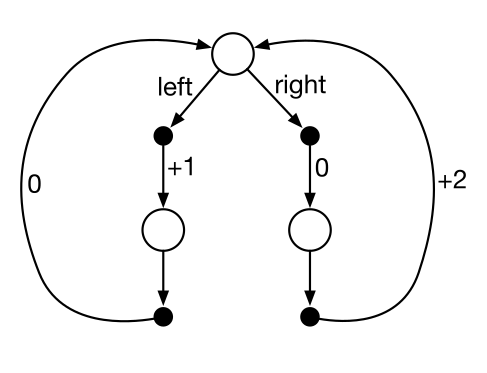
\includegraphics[width=0.4\linewidth]{./ex20.png}
\end{figure}
To find the optimal policy we first have to calculate the values of the two policies $v_{\pi_{left}}$ and $v_{\pi_{right}}$ in the various states of the MDP, which will here be called $s_0$ for the initial state, $s_l$ for the state after taking action \texttt{left} from $s_0$ and $s_r$ for the state after taking action \texttt{right} from $s_0$.
\begin{align*}
v_{\pi_{left}}(s_0) &=  \overbrace{p(s_l, 1 \mid s_0, \texttt{left} )}^{=1} [1 + \gamma\; v_{\pi_{left}}(s_l)] \\
v_{\pi_{left}}(s_0) &= 1 + \gamma\; (0 + \gamma\; v_{\pi_{left}}(s_0)) = 1 + \gamma^2 \; v_{\pi_{left}} \\
v_{\pi_{left}}(s_0) &= \frac{1}{1 - \gamma^2} \\ \\
v_{\pi_{left}}(s_l) &=  0 + \gamma\; v_{\pi_{left}}(s_0) \\
v_{\pi_{left}}(s_l) &=  \frac{\gamma}{1 - \gamma^2} \\ \\
v_{\pi_{left}}(s_r) &=  2 + \gamma\; v_{\pi_{left}}(s_0) \\
v_{\pi_{left}}(s_r) &= 2+ \frac{\gamma}{1 - \gamma^2} \\ \\
\end{align*}
And analogous for $v_{\pi_{right}}$:
\begin{align*}
v_{\pi_{right}}(s_0) &= 0 + \gamma \; v_{\pi_{right}}(s_r) \\
&= \gamma \; (2 + \gamma \; v_{\pi_{right}}(s_0)) \\
&= 2\gamma^2 + \gamma^2v_{\pi_{right}}(s_0) \\
v_{\pi_{right}}(s_0) &= \frac{2\gamma}{1 - \gamma^2} \\ \\
v_{\pi_{right}}(s_r) &= 2 + \gamma \; v_{\pi_{right}}(s_0) \\
v_{\pi_{right}}(s_r) &= 2 + \frac{2\gamma^2}{1-\gamma^2} = \frac{2}{1-\gamma^2} \\ \\
v_{\pi_{right}}(s_l) &= 0 + \gamma \; v_{\pi_{right}}(s_0) \\
v_{\pi_{right}}(s_l) &= \gamma \; \frac{2\gamma}{1-\gamma^2} = \frac{2\gamma^2}{1-\gamma^2} \\
\end{align*}
\begin{minipage}[t]{.3\textwidth}
\begin{tabular}{c|c|c|c}
$\gamma = 0$& $s_0$ & $s_l$ & $s_r$ \\ 
\hline 
$v_{\pi_{left}}$ & 1 & 0 & 2 \\ 
\hline 
$v_{\pi_{right}}$ & 0 & 0 & 2 \\ 
\end{tabular} 
\\ \\
As $v_{\pi_{left}} \geq v_{\pi_{right}}$ \\
$\rightarrow v_{\pi_{left}}$ optimal
\end{minipage}% <---------------- Note the use of "%"
\begin{minipage}[t]{.3\textwidth}
\begin{tabular}{c|c|c|c}
$\gamma=0.9$& $s_0$ & $s_l$ & $s_r$ \\ 
\hline 
$v_{\pi_{left}}$ & 5.25 & 4.74 & 6.74 \\ 
\hline 
$v_{\pi_{right}}$ & 9.47 & 8.53 & 10.53 \\ 
\end{tabular} \\ \\
As $v_{\pi_{right}} \geq v_{\pi_{left}}$ \\
$\rightarrow v_{\pi_{right}}$ optimal
\end{minipage}% <---------------- Note the use of "%"
\begin{minipage}[t]{.3\textwidth}
\begin{tabular}{c|c|c|c}
$\gamma = 0.5$ & $s_0$ & $s_l$ & $s_r$ \\ 
\hline 
$v_{\pi_{left}}$ & 1.33 & 0.67 & 2.67 \\ 
\hline 
$v_{\pi_{right}}$ & 1.33 & 0.67 & 2.67 \\ 
\end{tabular}\\ \\
As $v_{\pi_{left}} = v_{\pi_{right}}$ \\
$\rightarrow v_{\pi_{left}}$ and $v_{\pi_{right}}$ optimal
\end{minipage}% <---------------- Note the use of "%"

\subsection*{21. Exercise 3.24 Figure 3.5 (below) gives the optimal value of the best state of the gridworld as 24.4, to one decimal place. Use your knowledge of the optimal policy and (3.8) to express this value symbolically, and then to compute it to three decimal places.}
\begin{align*}
v_* (A) = \mathbf{max}_a\; \mathbb{E}_{\pi_*}[G_t \mid S_t = A, A_t = a]
\end{align*}
From Figure 3.5 we can see that the optimal policy directly leads from A' straight back to A, which gives a return of:
\begin{align*}
G_t &= R_{t+1} \gamma^0 + R_{t+2} \gamma ^1 + R_{t+3} \gamma ^2 + R_{t+4} \gamma ^3 + R_{t+5} \gamma^4 + R_{t+6} \gamma ^5 + ... \\
&= 10\gamma^0 + 0 \gamma ^1 + 0 \gamma ^2 + 0 \gamma ^3 + 0 \gamma^4 + 10 \gamma ^5 + ...\\
&= \sum_{k = 0}^\infty 10 \gamma^{5k} \\
&= 10 \sum_{k = 0}^\infty \gamma^{5k} \\
&= \frac{10}{1 - \gamma^5} \\
&\approx  24.419
\end{align*}
\newpage
\bibliographystyle{plainnat}
\bibliography{mybib}
\end{document}